\documentclass{article}

\usepackage[a4paper]{geometry}
\usepackage[T1]{fontenc}
\usepackage{graphicx}
\usepackage{amsmath}
\usepackage{amssymb}
\usepackage{listings}
\usepackage{xcolor}
\usepackage{booktabs}
\usepackage{parskip}
\usepackage{float}

\definecolor{gb_black}{HTML}{282828}
\definecolor{gb_gray}{HTML}{928374}
\definecolor{gb_red}{HTML}{cc241d}
\definecolor{gb_green}{HTML}{98971a}
\definecolor{gb_blue}{HTML}{458588}
\colorlet{background-color}{gb_gray!5}

\lstset{
    basicstyle=\color{gb_black}\ttfamily,
    keywordstyle=\color{gb_red},
    commentstyle=\color{gb_blue},
    stringstyle=\color{gb_green},
    numberstyle=\color{gb_black!35}\ttfamily,
    showspaces=false,
    showstringspaces=false,
    showtabs=false,
    columns=fullflexible,
    breaklines=true,
    postbreak=\mbox{\textcolor{gb_gray}{\(\hookrightarrow\)}\space},
    escapechar=\$,
    backgroundcolor=\color{background-color},
    numbers=none,
    frame=single,
    framerule=0pt,
}

\title{ECM2419: Software Development Coursework}
\author{730022096 \& 730002704}
\date{}

\begin{document}

    \maketitle


    \section{The V Model}
    We decided the best way to approach this project was by using the V-model as our software engineering lifecycle.
    This is a model where you first do the planning, preparation and documentation before you start any code, this is one of the key characteristics that distinguishes it from other software development models.

    We found many benefits in using this model including:
    \begin{enumerate}
        \item It is highly structured, and phases are completed one at a time.
        \item It works well for pair programming as all requirements are understood between everyone working on the code.
        \item It is simple to understand.
        \item It is easy to manage.
    \end{enumerate}


    \section{UML Diagram}
    The UML diagram of our finished production code is shown in Figure~\ref{fig:uml}.

    \begin{figure}[htbp]
        \centering
        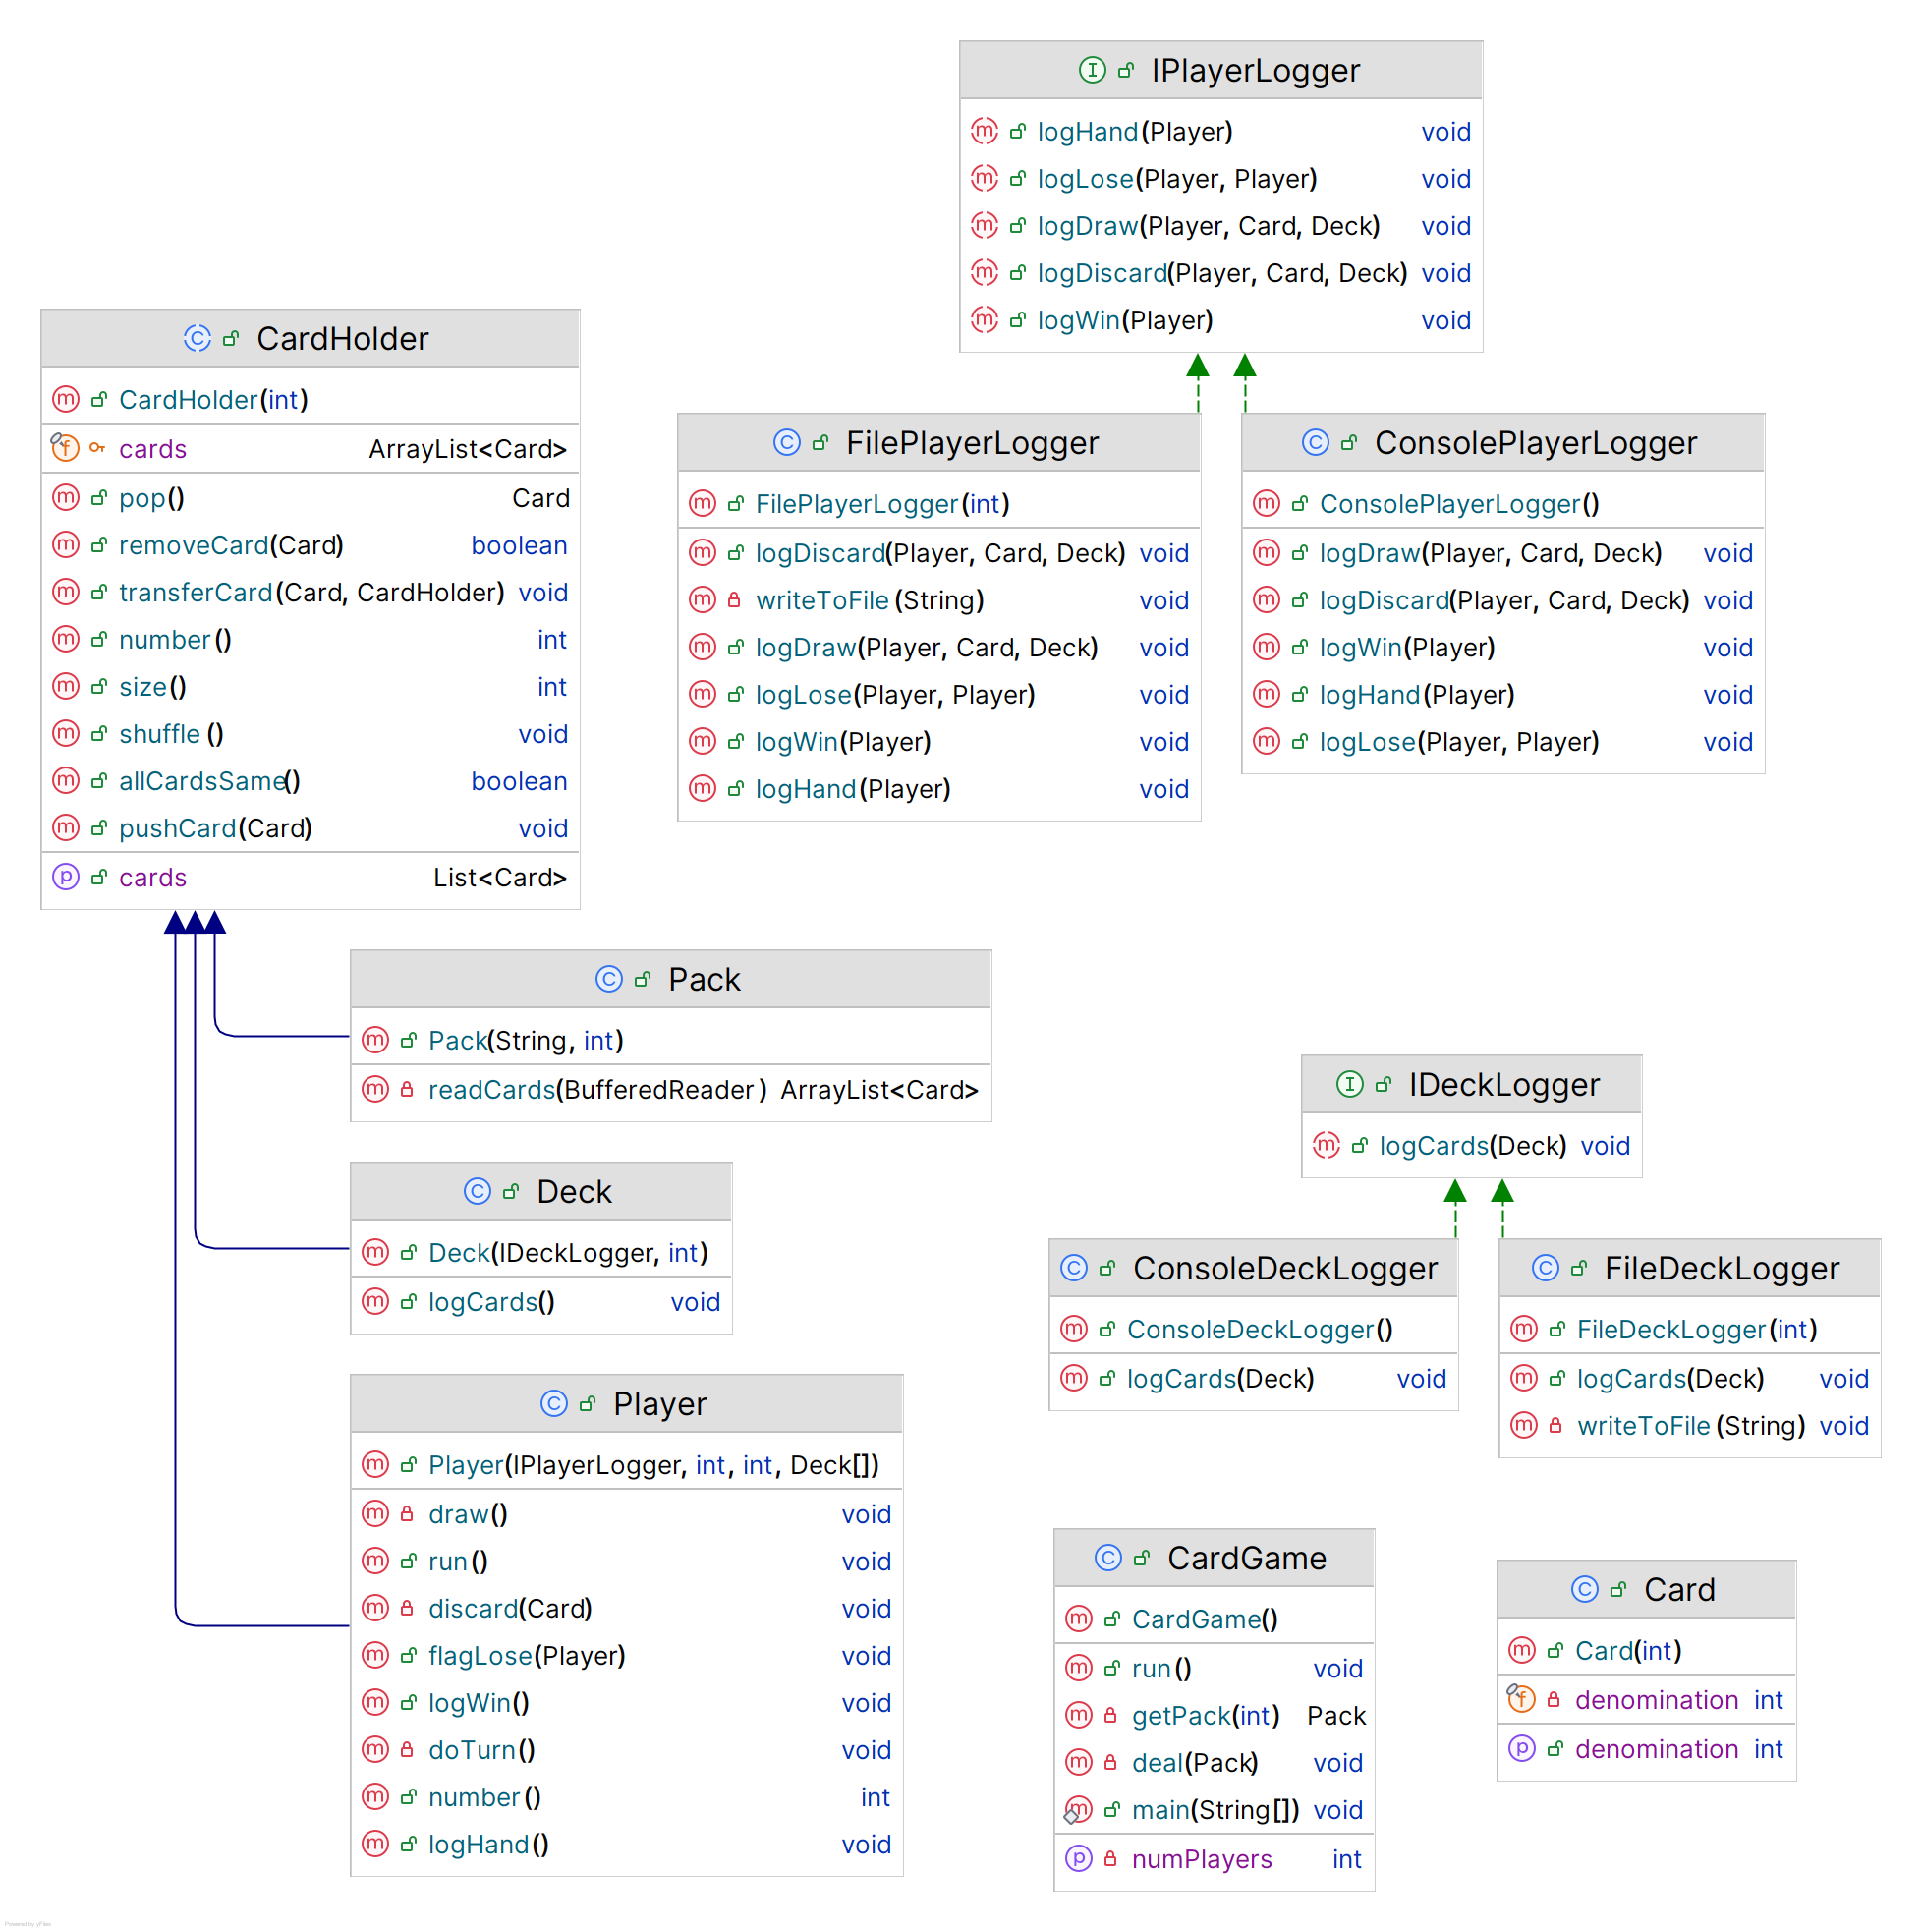
\includegraphics[width=.75\textwidth]{uml}
        \caption{UML Diagram.}
        \label{fig:uml}
    \end{figure}

    In this UML diagram you can see that we used a structural design pattern and more specifically this would be the Facade design pattern.

    The facade design pattern provides a simplified interface to a complex subsystem.
    In our case, the high-level classes like \texttt{IPlayerLogger}, \texttt{IDeckLogger}, and \texttt{CardGame} act as the facade providing an interface to the underlying subsystems and components.


    \section{Key Design Choices}

    \subsection{Facade Design Pattern}
    We decided to use a pattern like this as it provided a simplified and consistent interface to the more complex game logic and all the other complex number/data management components going on as well.

    \subsection{Class Hierarchy}
    In our design we used high-level parent classes like \texttt{IPlayerLogger}, \texttt{IDeckLogger}, and \texttt{CardHolder} that encapsulate the functionality and are extended by more specialized classes like \texttt{ConsolePlayerLogger}, \texttt{FilePlayerLogger}, and \texttt{CardHolder}.

    We did this as it promotes the separations of concerns and makes the code easier to understand which then makes it easier to maintain and whilst we were still editing the code it makes it easier to extend any code where we need to.

    \subsection{Separation of Concerns}
    Another key point of our design is Separation of Concerns.
    The design separates different responsibilities into distinct classes: e.g.\ Card: Data structure, Deck: Card collection management etc.
    The benefits of doing this include:
    \begin{enumerate}
        \item Easy to maintain and modify.
        \item Clear responsibilities for each component.
        \item Reduced coupling between components.
        \item Better for paired programming.
        \begin{enumerate}
            \item Makes it easier to work on different parts of the code at the same time.
            \item Makes it easier to understand the code.
        \end{enumerate}
    \end{enumerate}

    \subsection{Logging and Debugging}
    Using the logger classes \texttt{IPlayerLogger}, \texttt{IDeckLogger}, and \texttt{ConsolePlayerLogger} gives us more of a focus on logging and debugging functionality.

    We did this as it is useful for tracking and analysing game events, player actions, and potential issues during our development of the project.


    \section{Testing}

    \subsection{CardHolderTest}

    \subsubsection{Test Coverage}
    \begin{itemize}
        \item Testing of \texttt{CardHolder} methods
        \item Tests both successful and edge cases
    \end{itemize}
    We wanted a range of tests that could test all methods in the \texttt{CardHolder} class effectively and efficiently and follow all the attributes of the Right Bicep test planning model. With that in mind, we designed the tests:
    \begin{itemize}
        \item \texttt{pushCard()}
        \begin{itemize}
            \item Tests adding a card to a \texttt{CardHolder}
        \end{itemize}
        \item \texttt{popCard()}
        \begin{itemize}
            \item Tests removing the top card from a \texttt{CardHolder}
        \end{itemize}
        \item \texttt{popCard\_empty()}
        \begin{itemize}
            \item Tests attempting to pop a card from an empty \texttt{CardHolder}
        \end{itemize}
        \item \texttt{removeCard()}
        \begin{itemize}
            \item Tests removing a specific card from a \texttt{CardHolder}
        \end{itemize}
        \item \texttt{removeCard\_nonExistent()}
        \begin{itemize}
            \item Tests removing a card not in the \texttt{CardHolder}
        \end{itemize}
        \item \texttt{transferCard()}
        \begin{itemize}
            \item Tests transferring a card between two Card Holders
        \end{itemize}
        \item \texttt{transferCard\_nonExistent()}
        \begin{itemize}
            \item Tests transferring a non-existent card
        \end{itemize}
        \item \texttt{allCardsSame()}
        \begin{itemize}
            \item Tests checking if all cards in a \texttt{CardHolder} have the same denomination
        \end{itemize}
        \item \texttt{allCardsSame\_empty()}
        \begin{itemize}
            \item Tests \texttt{allCardsSame()} method on an empty \texttt{CardHolder}
        \end{itemize}
        \item \texttt{getCards()}
        \begin{itemize}
            \item Tests retrieving the list of cards from a \texttt{CardHolder}
        \end{itemize}
    \end{itemize}

    \subsubsection{Error Handling}
    \begin{itemize}
        \item We used \texttt{@Test(expected = IllegalStateException.class)} for error scenarios
        \item Verifies correct behaviour when attempting operations on empty collections
    \end{itemize}

    \subsubsection{State Validation}
    \begin{itemize}
        \item Checks list size after operations
        \item Verifies correct card placement and transfer
        \item Ensures state consistency after each operation
    \end{itemize}

    \subsubsection{Setup Strategy}
    \begin{itemize}
        \item We used \texttt{@Before} annotation to create new CardHolder instances for each test
        \item Creates two separate CardHolder instances to test interactions
    \end{itemize}

    \subsection{CardTest}
    Single test method for \texttt{getDenomination()} with basic verification of Card object's core functionality.

    \subsection{PackTest}

    \subsubsection{Test Coverage}
    \begin{itemize}
        \item \texttt{testPackCreation\_ValidFile()}
        \begin{itemize}
            \item Tests creating a Pack with a valid file containing 16 cards
        \end{itemize}
        \item \texttt{testPackCreation\_InvalidFile\_NotEnoughLines()}
        \begin{itemize}
            \item Tests creating a Pack with a file that has insufficient lines
        \end{itemize}
        \item \texttt{testPackCreation\_InvalidFile\_NonIntegerValue()}
        \begin{itemize}
            \item Tests creating a Pack with a file containing a non-integer value
        \end{itemize}
        \item \texttt{testPop\_ValidCase()}
        \begin{itemize}
            \item Tests the \texttt{pop()} method of the Pack - Verifies the first card has the correct denomination (1)
        \end{itemize}
        \item \texttt{testPackCreation\_EmptyFile()}
        \begin{itemize}
            \item Tests creating a Pack with an empty file
        \end{itemize}
    \end{itemize}

    \subsubsection{File-Based Testing}
    \begin{itemize}
        \item We used temporary file creation for testing Pack initialization
        \item Tests multiple file input scenarios
        \item Dynamically generates test files with different contents
    \end{itemize}

    \subsubsection{Error Scenario Coverage}
    \begin{itemize}
        \item Tests pack creation with:
        \begin{itemize}
            \item Valid file
            \item Insufficient lines
            \item Non-integer values
            \item Empty file
        \end{itemize}
    \end{itemize}

    \subsubsection{File Handling}
    \begin{itemize}
        \item Implements a helper method \texttt{createTemporaryPackFile()} to manage test file creation
        \item Uses try-with-resources for safe file writing
        \item We used \texttt{java.nio.file} for temporary file management
    \end{itemize}

    \subsection{Design Choices}
    \begin{itemize}
        \item Follows JUnit testing conventions
        \item Uses \texttt{assertXXX} methods for validation
        \item Tests both successful and failure paths
        \begin{itemize}
            \item Leads to more accurate testing results
        \end{itemize}
        \item We focused on individual method behaviour
        \begin{itemize}
            \item Means we can get more accurate test results and accurately test that each method is working how it is designed
        \end{itemize}
        \item Ensures predictable object state after operations
        \item Uses \texttt{@Before} annotation to create new instances for each test
        \begin{itemize}
            \item Means we can accurately test each method more accurately to ensure the functionality is working properly
        \end{itemize}
    \end{itemize}


    \section{Work Log}
    \begin{table}[H]
        \centering
        \begin{tabular}{llll}
            \toprule
            \textbf{Date} & \textbf{Hours} & \textbf{730022096} & \textbf{730002704} \\
            \midrule
            24/8/24       & 3              & Documentation      & Documentation      \\
            29/10/24      & 3              & Driver             & Observer           \\
            5/11/24       & 3              & Observer           & Driver             \\
            7/11/24       & 2              & Driver             & Observer           \\
            14/11/24      & 4              & Observer           & Driver             \\
            21/11/24      & 4              & Driver             & Observer           \\
            28/11/24      & 3              & Observer           & Driver             \\
            1/12/24       & 4              & Driver             & Observer           \\
            5/12/24       & 4              & Observer           & Driver             \\
            \bottomrule
        \end{tabular}
        \caption{Work Log.}
        \label{tab:work-log}
    \end{table}

\end{document}
